\section{Constant Density Flow}
For the profile in \eqref{ho:pro2} with constant density
$\rho=\rho_0$ everywhere, the trial solution of the Reyleigh's
Stability equation \eqref{kh:ray2} is in the form
\begin{equation}\label{hom:con0}
\phi =
\begin{cases}
Ae^{-\alpha z} &\text{if $z>1$,}\\
Be^{-\alpha z} + Ce^{\alpha z} &\text{if $-1<z<1$,}\\
De^{\alpha z} &\text{if $z<-1$.}
\end{cases}
\end{equation}

At $z=1$, the boundary conditions are:
\begin{enumerate}
  \item[(i)] pressure:
  \begin{align}
    \hat{p}&=U'\phi-(U-c)\phi'\quad \text{is continuous}\notag\\
    -(1-c)Ae^{-\alpha}&=Be^{-\alpha} + Ce^{\alpha}-(1-c)\alpha(-B
    e^{-\alpha}+Ce^{\alpha})\label{hom:con1}
  \end{align}
  \item[(ii)] displacement:
  \begin{align}
    \phi &\quad \text{is continuous}\notag\\
    Ae^{-\alpha}&=Be^{-\alpha} + Ce^{\alpha}\label{hom:con2}
  \end{align}
\end{enumerate}
Substitute \eqref{hom:con2} into \eqref{hom:con1}, I get
\begin{equation}\label{hom:con3}
    2(1-c)\alpha C=Be^{-2\alpha}+C
\end{equation}

At $z=-1$, the boundary conditions are:
\begin{enumerate}
  \item[(i)] pressure:
  \begin{equation}
    -(-1-c)Ae^{\alpha}=Be^{\alpha} + Ce^{-\alpha}-(-1-c)\alpha(-B
    e^{\alpha}+Ce^{-\alpha})\label{hom:con4}
  \end{equation}
  \item[(ii)] displacement:
  \begin{equation}
    Be^{\alpha} + Ce^{-\alpha}=De^{\alpha}\label{hom:con5}
  \end{equation}
\end{enumerate}
Substitute \eqref{hom:con5} into \eqref{hom:con4}, I get
\begin{equation}\label{hom:con6}
    2(1+c)\alpha B=B+Ce^{-2\alpha}
\end{equation}

Combining \eqref{hom:con3} and \eqref{hom:con6} to eliminate the
constants $B$ and $C$, I found that the non-dimensional phrase speed
satisfy the equation:
\begin{equation}\label{hom:con}
    \boxed{c^2+\Bigl(\frac{e^{-4\alpha}-(2\alpha-1)^2}{4\alpha^2}\Bigr)=0}
\end{equation}
The solution is
\begin{equation}\label{hom:con7}
    c=\pm\sqrt{\Bigl(1-\frac{1}{2\alpha}\Bigr)^2-\Bigl(\frac{1}{4\alpha^2}\Bigr)e^{-4\alpha}}
\end{equation}

The value of $\alpha$ was solved numerically. For $\alpha>0.639232$,
$c$ is real, the solution is neutral. For $0\leq\alpha\leq0.639232$,
$c$ is imaginary, one of the solutions is unstable. The value of
$c_R$ and $c_I$ is plotted in Figure \ref{ho1} and \ref{ho2}. From
the graph we can verify that when $\alpha \rightarrow 0$, $c=\pm i$,
this recovers the result of Kelvin-Helmholtz instability.
\begin{figure}[htpb]
  \centering
  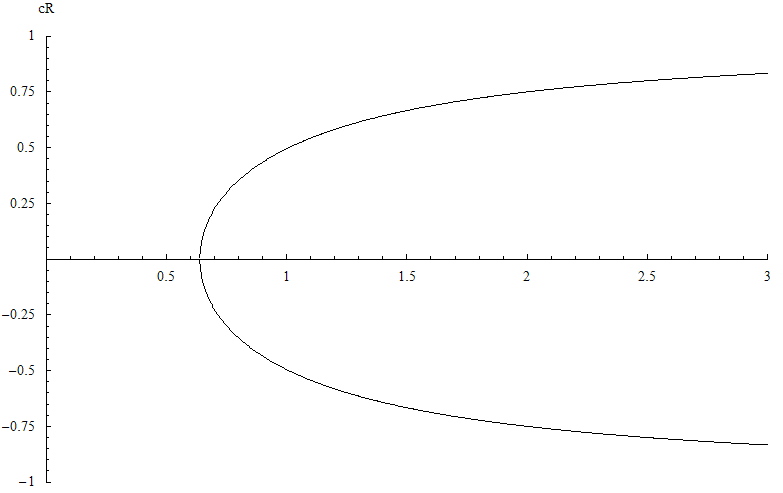
\includegraphics[width=0.9\textwidth]{ho1.png}\\
  \caption{$c_R$ vs.~$\alpha$ for $U_0=1$ of a Holmboe mode}\label{ho1}
\end{figure}
\begin{figure}[htpb]
  \centering
  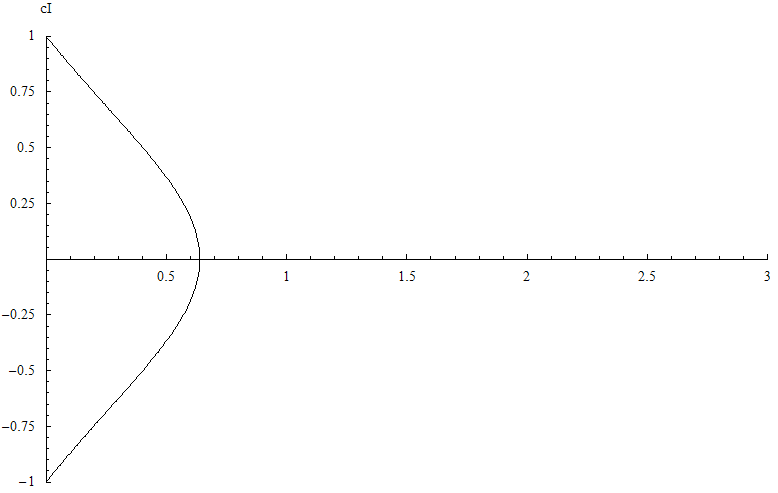
\includegraphics[width=0.9\textwidth]{ho2.png}\\
  \caption{$c_I$ vs.~$\alpha$ for $U_0=1$ of a Holmboe mode}\label{ho2}
\end{figure}
